\chapter{Governing Equations}
\label{chap:governing}

This chapter focuses on the equations governing viscous plane flows, and moves on to manipulating these equations to derive the famous \emph{Orr-Sommerfeld equation}, a famous eigenvalue equation for linear stability that (as we will see later in the report) can be solved to determine the stability of a flow. This chapter also introduces the two types of viscous plane flow this report deals with, plane Poiseuille flow and plane Couette flow. 

\section{Basic state and governing equations}
\textbf{check the notation used for the dimensional v dimensionless cases, make sure it is consistent}

A plane flow is a 2-dimensional flow represented by a velocity profile $ U $ in a single direction. For this project, we will consider $ U $ that are functions of $ z $ only and act in the $ x $ direction. Moreover, our flow will be considered to be flowing through a 'channel' that is bounded between $ z = z_{1_*} $ and $ z = z_{1_*} $.

We denote our basic steady flow as
\begin{equation}
    \mathbf{U}_* = U_* (z_*) \mathbf{i} \hspace{10px} (z_{1_*} \leq z_* \leq z_{2_*}),
\end{equation}
with boundaries on $z_* = z_{1_*} \text{and } z_{2_*}$ that are either \emph{rigid} or \emph{free}:
\begin{itemize}
    \item \emph{rigid} - normal component of velocity must vanish
    \item \emph{free} - pressure must be constant
\end{itemize}

The governing equations for this system are the same as any viscous flow, the continuity equation and the Navier-Stokes equation for an incompressible fluid. 
\begin{align}
    \div{\mathbf{u_*}} &= 0, \nonumber\\
    \pdv{\mathbf{u_*}}{t_*} + \mathbf{u_*} \cdot \nabla \mathbf{u_*} &= - \frac{1}{\rho} \nabla p_* + \nu \Delta \mathbf{u_*}.
\label{dimgoveq}
\end{align}

Note that we denote the \emph{kinematic viscosity} $ \nu = \frac{\mu}{\rho} $ and have also set $ f = 0 $ in the Navier-Stokes equation, assuming there is no force acting on the fluid. The fluid discussed in this report is also considered to have a constant density i.e. $ \rho = \text{const.} $

Figure \ref{fig:pflow} shows a schematic of the system we will be analysing in an initial stable state. 

\begin{figure}[htb!]
    \centering
    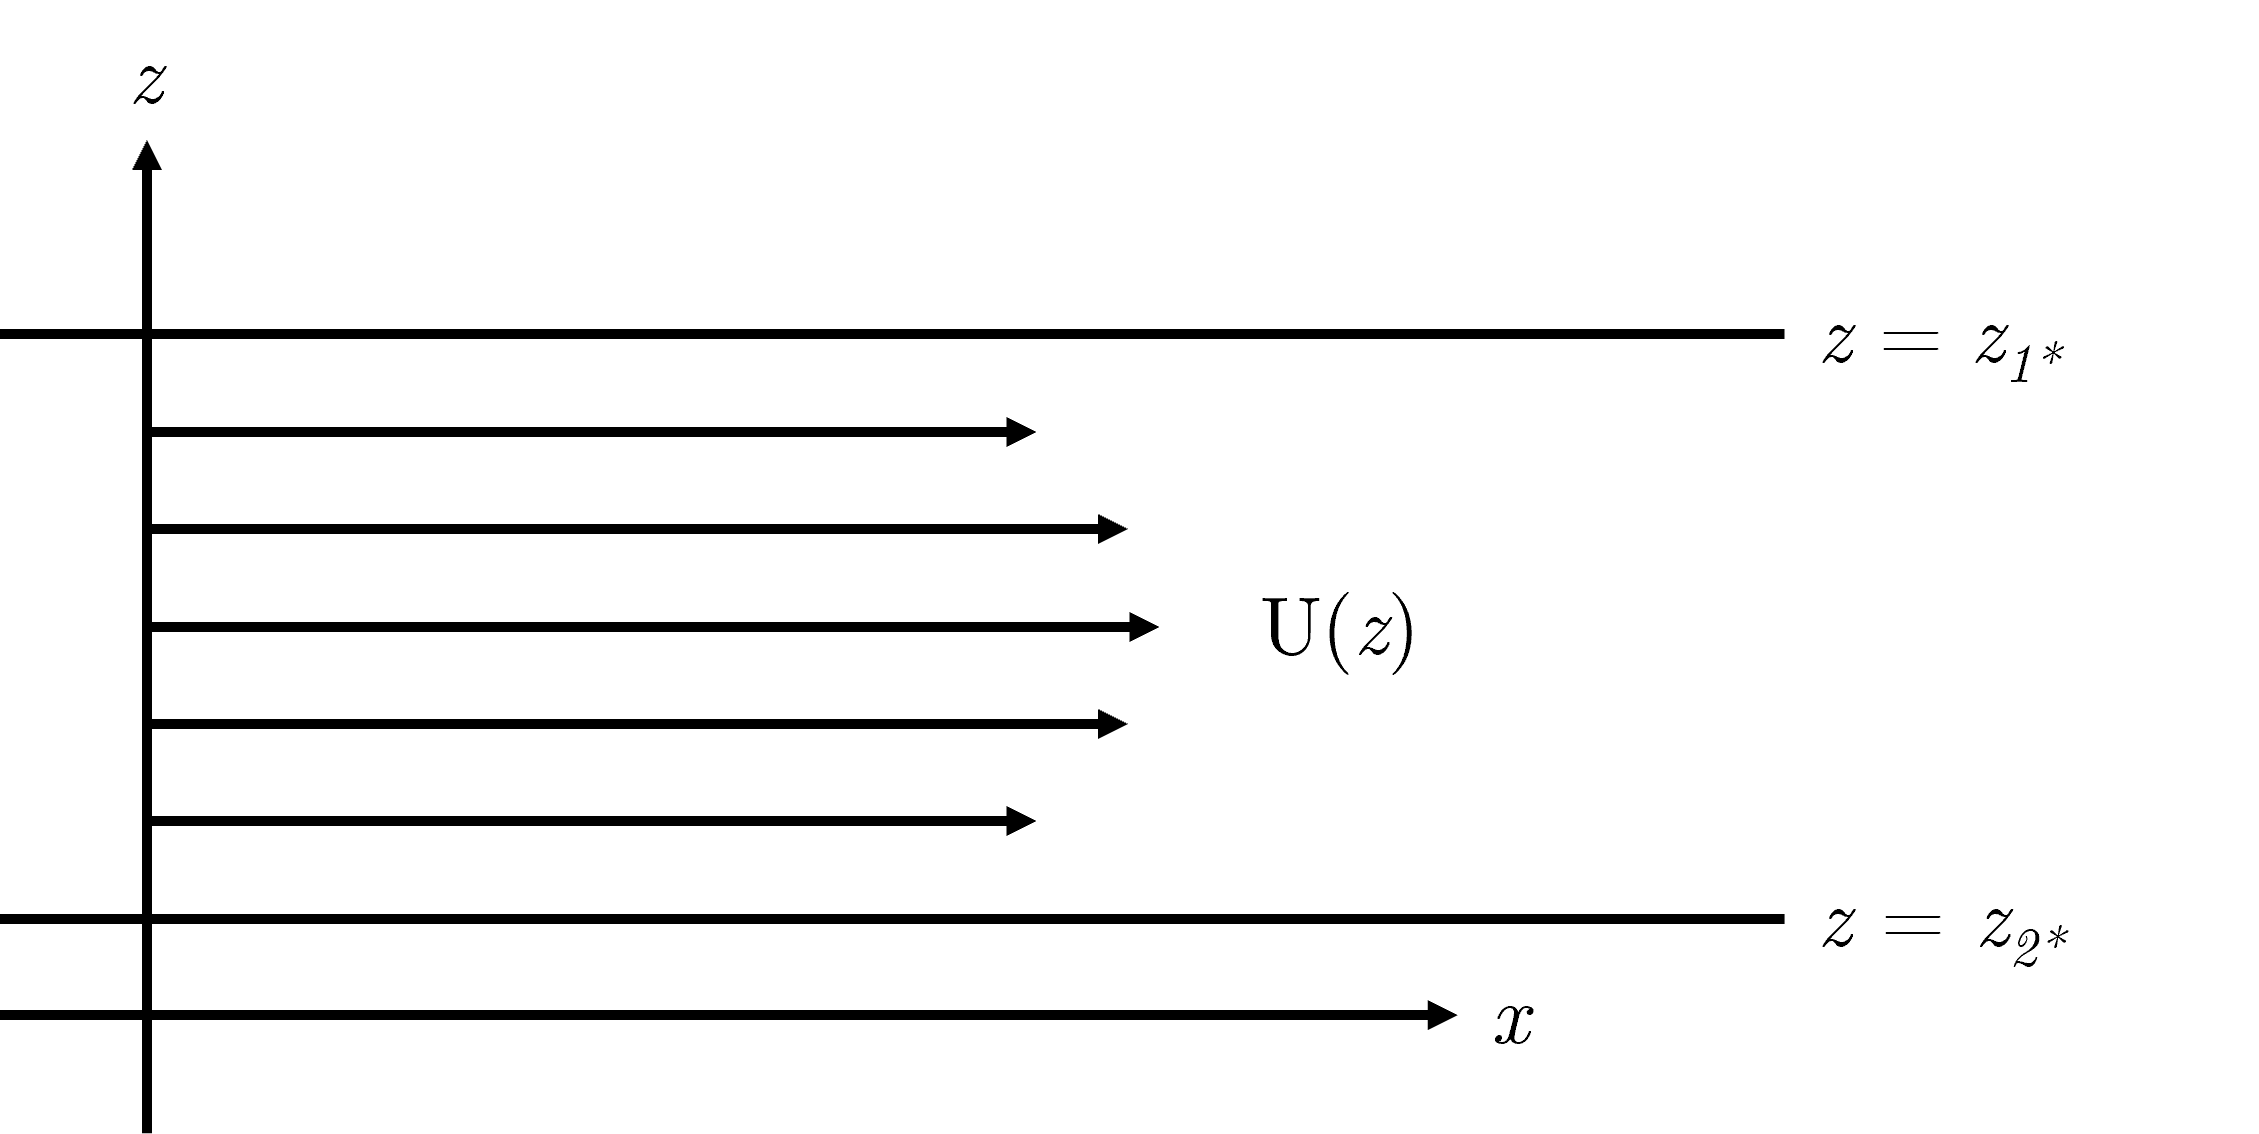
\includegraphics[width=10cm]{figures/PSF.png}
    \caption{The setup of our flow}
    \label{fig:pflow}
\end{figure}

\section{Dimensionless Governing Equations}

We would like to get a dimensionless form of our governing equations \eqref{dimgoveq}. This is useful because it allows us to map our flow to a corresponding flow of width $ z = - 1 $ to $ z= 1$. As we will see later in this chapter, this allows us to analyse families of flows that have an equivalent Reynolds number. In Chapter \ref{chap:numerics} we will also see that this range is the same as the range of the Chebyshev polynomials that are fundamental to our numerical solution.

To write the governing equations in terms of dimensionless quantities we utilise the following change of variables as in \citet{drazin2004hydrodynamic}: 
\begin{align}
    t = \frac{t_* V}{L},\ \mathbf{x} &= \frac{\mathbf{x_*}}{L},\ \mathbf{u} = \frac{\mathbf{u_*}}{V},\ p = \frac{p}{\rho V^2}, \nonumber\\ \mathbf{U} &= \frac{\mathbf{U_*}}{V} \equiv U(z) \mathbf{i},
\end{align}
where we refer to $ V $ as the \emph{characteristic velocity} and $ L $ as the \emph{characteristic length}, defined as
\begin{align}
    V &= \text{max}_{z_* \in [z_{1_*}, z_{2_*}]} |U_* (z_*)|, \nonumber\\
    L &= \tfrac{1}{2}(z_{2_*} - z_{1_*}).
\end{align}

So in this case, the characteristic velocity of a flow is the maximum velocity of its initial velocity profile and the characteristic length is half the width of the channel. Note that the basic flow still acts in just the $ x $ direction, meaning that the dimensionless flow still has the same form as in Figure \ref{fig:pflow}.

We can now use this transformation to find dimensionless forms of the various derivatives in the governing equations. By the chain rule, we have
\begin{equation}
    \pdv{\mathbf{u}}{t} = \pdv{\mathbf{u}}{\mathbf{u_*}} \pdv{\mathbf{u_*}}{t_*} \pdv{t_*}{t} = \frac{L}{V^2} \pdv{\mathbf{u_*}}{t_*} \implies \pdv{\mathbf{u_*}}{t_*} = \frac{V^2}{L} \pdv{\mathbf{u}}{t},
\label{dut*}
\end{equation}
and
\begin{gather}
    (\nabla \mathbf{u_*})^\mu = \pdv{\mathbf{u_*}}{{x_*}^\mu} = \pdv{\mathbf{u_*}}{\mathbf{u}} \pdv{\mathbf{u}}{x^\mu} \pdv{x^\mu}{{x_*}^\mu} = \frac{V}{L} \pdv{\mathbf{u}}{x^\mu} = \frac{V}{L} (\nabla \mathbf{u})^\mu \nonumber\\
    \implies \nabla \mathbf{u_*} = \frac{V}{L} \nabla \mathbf{u}.
\label{gradu*}
\end{gather}

\textbf{the below needs updating I think or some explanation of what is being done here}

Similarly,
\begin{gather}
    (\Delta \mathbf{u_*})^\mu = \pdv{{x_*}^\mu} (\nabla \mathbf{u_*})^\mu = \frac{1}{L} \pdv{x^\mu}(\frac{V}{L} (\nabla \mathbf{u})^\mu) = \frac{V}{L^2} (\Delta \mathbf{u})^\mu \nonumber\\
    \implies \Delta \mathbf{u_*} = \frac{V}{L^2} \Delta \mathbf{u},
\label{lapu*}
\end{gather}
and
\begin{gather}
    \div{\mathbf{u_*}} = \pdv{{u_*}^\mu}{{x_*}^\mu} = \frac{V}{L} \pdv{u^\mu}{x^\mu} = \frac{V}{L} \div{\mathbf{u}}.
\label{divu*}
\end{gather}
Finally, for $ p_* $ we need just $ \nabla p_* $ in terms of $ \nabla p $, again using the chain rule we obtain
\begin{gather}
    (\nabla p_*)^\mu = \pdv{p_*}{{x_*}^\mu} = \pdv{p_*}{p} \pdv{p}{x^\mu} \pdv{x^\mu}{{x_*}^\mu} = \rho V^2 \pdv{p}{x^\mu} \frac{1}{L} = \frac{\rho V^2}{\mu} \pdv{p}{x^\mu} \nonumber\\
    \implies \nabla p_* = \frac{\rho V^2}{L} \nabla 
\label{gradp*}
\end{gather}
We can now substitute these results into our governing equations \eqref{dimgoveq} to get their dimensionless forms. For the \emph{continuity equation} we use equation \eqref{divu*} to get
\begin{gather}
    0 = \div{\mathbf{u_*}} = \frac{V}{L} \div{\mathbf{u}} \implies \div{\mathbf{u}} = 0.
\end{gather}
Substituting our remaining equations \eqref{dut*}, \eqref{gradu*}, \eqref{lapu*}, \eqref{gradp*} into the \emph{Navier-Stokes equation} we get
\begin{align}
        \pdv{\mathbf{u_*}}{t_*} + \mathbf{u_*} \cdot \nabla \mathbf{u_*} &= - \frac{1}{\rho} \nabla p_* + \nu \Delta \mathbf{u_*} \nonumber\\
        \implies \frac{V^2}{L} \pdv{\mathbf{u}}{t} + (V \mathbf{u}) \cdot (\frac{V}{L}\nabla \mathbf{u}) &= - \frac{1}{\rho} (\frac{\rho V^2}{L} \nabla p) + \nu (\frac{V}{L^2} \Delta \mathbf{u}) \nonumber\\
        \implies \frac{V^2}{L} \pdv{\mathbf{u}}{t} + \frac{V^2}{L} \mathbf{u} \cdot \nabla \mathbf{u} &= -\frac{V^2}{L} \nabla p + \frac{\nu V}{L^2} \Delta \mathbf{u} \nonumber\\
        \implies \pdv{\mathbf{u}}{t} + \mathbf{u} \cdot \nabla \mathbf{u} &= -\nabla p + \frac{\nu}{V L} \Delta \mathbf{u}
\end{align}
Notice that $ \frac{V L}{\nu} $ is the famous \emph{Reynolds number} $ R $. Using this in the Navier-Stokes equation leaves us with our pair of \emph{dimensionless governing equations}
\begin{align}
    \div{\mathbf{u}} &= 0, \nonumber\\
    \pdv{\mathbf{u}}{t} + \mathbf{u} \cdot \nabla \mathbf{u} &= -\nabla p + R^{-1} \Delta \mathbf{u}.
\label{dlessgoveq}
\end{align}

If we substitute our basic flow $ \mathbf{u}(\mathbf{x}, t) = U(z) \mathbf{i} $ and basic pressure, $ p (\mathbf{x}, t) = P(\mathbf{x}) $ into \eqref{dlessgoveq}, we find that $ U(z) $ must satisfy the following equation of motion 
\begin{equation}
    \dv[2]{U}{z} = R \dv{P}{x}
\end{equation}
which limits our choices of $ U (z) $ and $ P (\mathbf{x})$. There are two main important cases defined as follows:
\begin{list}{$-$}{\leftmargin=1cm}
    \item \emph{Poiseuille flow}: $ U(z) = 1 - z^2 $ with $ \dv{P}{x} = const. $
    \item \emph{Couette flow}: $ U(z) = z $ with $ P = const. $
\end{list}

Schematic diagrams for these 2 flows can be seen in Figure \ref{fig:pandcflow}. Poiseuille flow can be thought of as representing a velocity being applied in the centre of the channel, or the fluid 'sticking' at the edges. This is common with more viscous fluids. Couette flow on the other hand can be thought of as a representation of the flow 'shearing.'

% This leaves us with a family of flows to analyse formed by a linear combination of these 2 types of flow.

\begin{figure}[htb!]
    \centering
    \subfloat[Poiseuille flow]{
    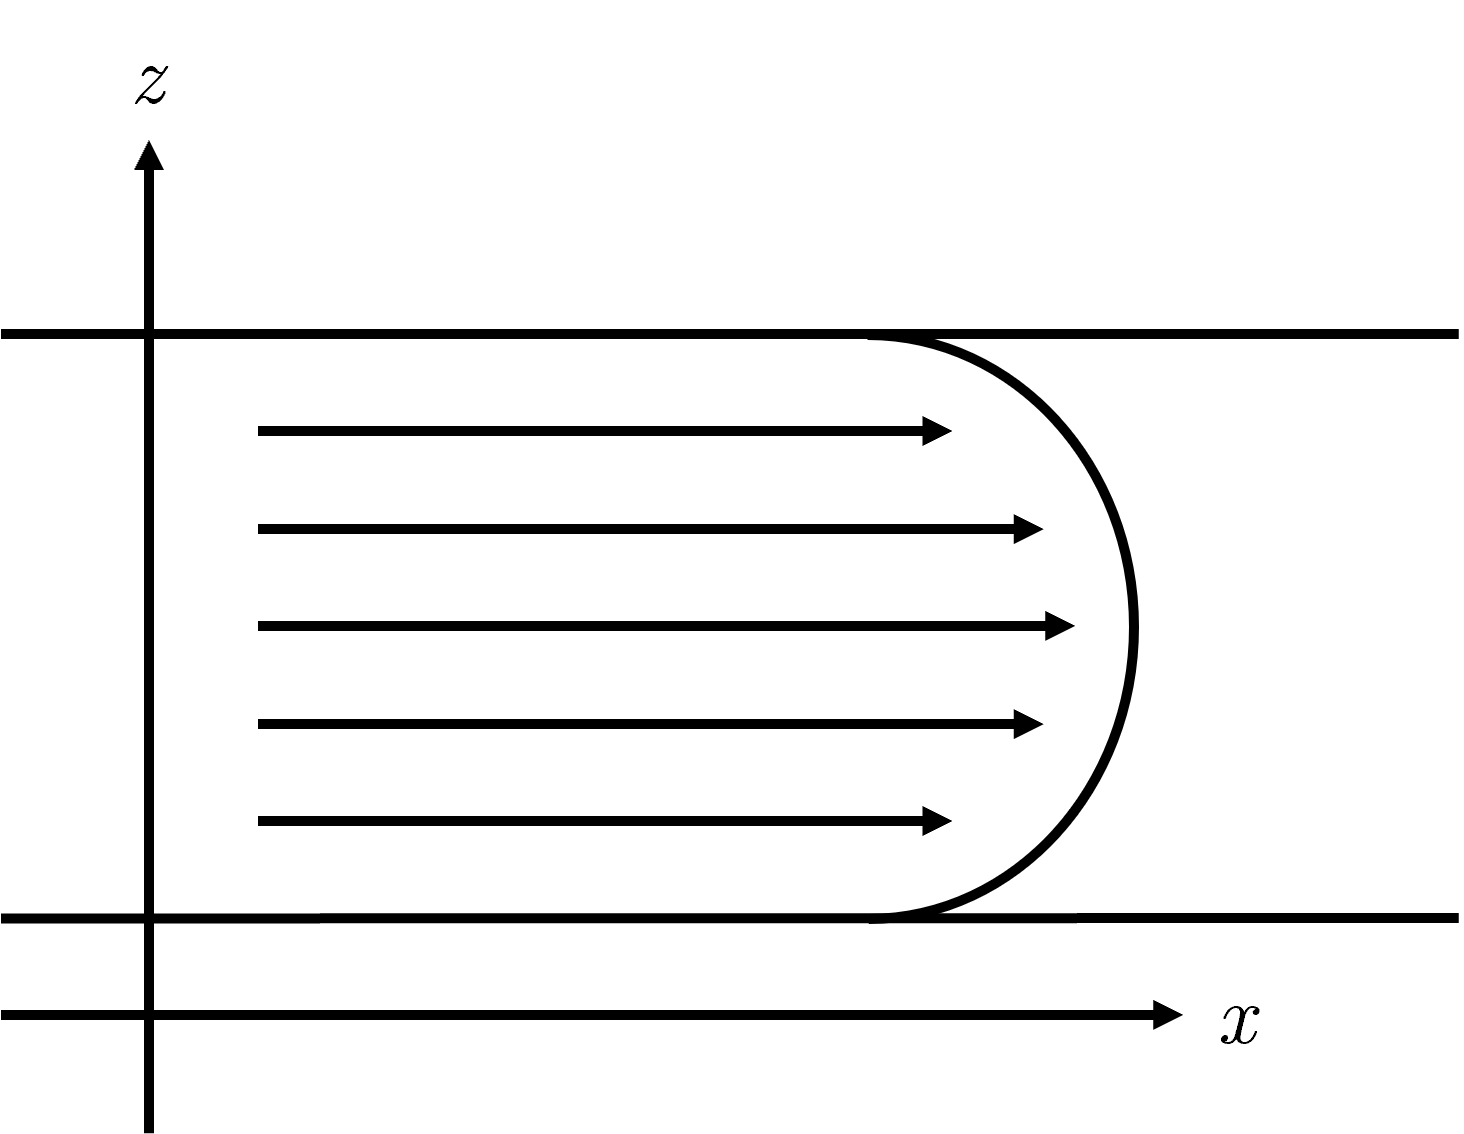
\includegraphics[width=80mm]{figures/PoiseuilleFlow.png}
    }
    \subfloat[Couette flow]{
    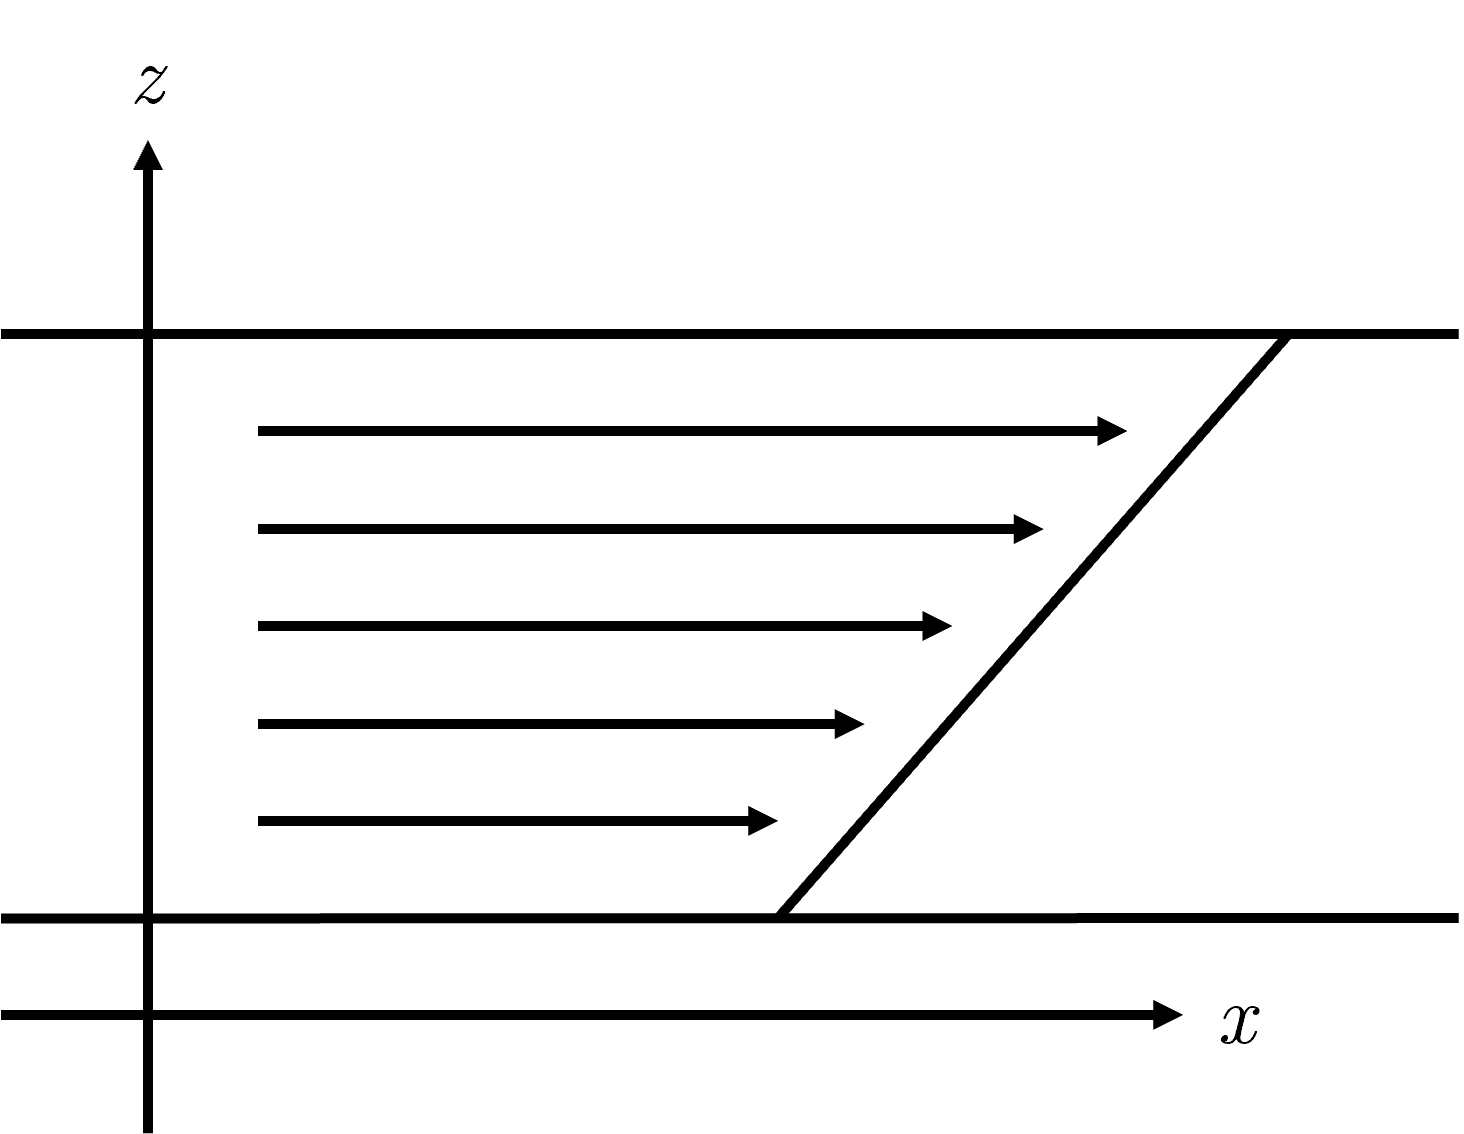
\includegraphics[width=80mm]{figures/CouetteFlow.png}
    }
    \caption{Schematics of plane Poiseuille and plane Couette flow}
    \label{fig:pandcflow}
\end{figure}

Before we move on to linearising our governing equations, a discussion of the Reynolds number is in order. As we can see it provides a ratio between the three main variables that define our flow: the velocity, width and viscosity. It scales proportionally to width and velocity, but inversely proportional to viscosity. This means a flow with a high Reynolds number could have one of three things: it could be travelling at a high velocity, be flowing through a very wide channel, or have a low viscosity. This means an example of a flow with a high Reynolds number could be: a flow of water or alcohol which has a low viscosity, a flow with a large channel such as a wide section of river, or a fluid being pumped quickly such as fuel being transported through a pipe. A flow with a low Reynolds number might have a high viscosity fluid, be travelling slowly or be travelling through a thinner channel. This means a flow of a fluid like honey could have a low Reynolds number.

If we can find conditions on the Reynolds number that relate to stability then this may tell us what these parameters should be set to proportional to each other. For example, if flows with a high Reynolds number are more stable, then for a more viscous flow we may want to increase the width of the channel it is being pumped through to increase its stability. If flows of a low Reynolds number are more stable, then we may want to decrease the width of the channel for flow with lower viscosity.

\section{Linearising the governing equations}

To study the stability of a plane flow we consider small perturbations to $ \mathbf{u} $ and $ p $ of the form
\begin{align}
    \mathbf{u}(\mathbf{x}, t) &= U(z) \mathbf{i} + \mathbf{u}'(\mathbf{x}, t), \nonumber\\
    p(\mathbf{x}, t) &= P(\mathbf{x}) + p'(\mathbf{x}, t).
\end{align}

We can now substitute these equations back into our dimensionless governing equations \eqref{dlessgoveq}. From here we linearise, discarding any terms that are non-linear in  $ \mathbf{u}' $ or  $ p' $. Note that this means that for the remainder of this report we are analysing the linear stability of a flow as all non-linear components have been removed. This has some impact on the validity of our report, as we will see when we come to discussing our results later on.

For the continuity equation we get
\begin{equation}
    0 = \div{\mathbf{u}} =  \div{( U \mathbf{i} + \mathbf{u}'(\mathbf{x}, t))} = \div{\mathbf{u}'}
\label{contlin}
\end{equation} 
where the term $ \div{U \mathbf{i}} $ vanishes as $ U $ is a function of $ z $ only.
For the Navier-Stokes equation, we linearise the individual terms separately for readability. 

For $ \pdv{\mathbf{u}}{t} $, 
\begin{equation}
    \pdv{\mathbf{u}}{t} = \pdv{t} (U(z) \mathbf{i} + \mathbf{u}'(\mathbf{x}, t)) = \pdv{\mathbf{u}'}{t}.
\end{equation}
Similarly
\begin{align}
    \mathbf{u} \cdot \nabla \mathbf{u} &= (U \mathbf{i} + \mathbf{u}' (\mathbf{x}, t)) \cdot \nabla (U \mathbf{i} + \mathbf{u}' (\mathbf{x}, t)) \nonumber\\
    &= (U \mathbf{i} + \mathbf{u}' (\mathbf{x}, t)) \cdot (\nabla \mathbf{u}' + \nabla U) \nonumber\\
    &= U \mathbf{i} \cdot \nabla \mathbf{u}' + \mathbf{u}' \cdot \nabla \mathbf{u}' + \mathbf{u}' \nabla U \mathbf{i} + U \mathbf{i} \cdot \nabla U \mathbf{i}.
\end{align}
We now omit $ \mathbf{u}' \cdot \nabla \mathbf{u}' $ as it is quadratic in $ \mathbf{u}' $. We are left with
\begin{equation}
    \mathbf{u} \cdot \nabla \mathbf{u} = U \pdv{\mathbf{u}'}{x} + w' \frac{\text{d}U}{\text{d}z} \mathbf{i},
\end{equation}
where $ w' $ represents the $ z$-component of $ \mathbf{u}'$. For the right hand side we get
\begin{align}
    \nabla p &= \nabla (P(\mathbf{x}) + p') = -\nabla p', \nonumber\\
    \Delta \mathbf{u} &= \Delta (U \mathbf{i} + \mathbf{u}' (\mathbf{x}, t)) \nonumber\\
    &= \div{\nabla (U \mathbf{i} + \mathbf{u}' (\mathbf{x}, t))} \nonumber\\
    &= \div{\nabla \mathbf{u}'} = \Delta \mathbf{u}'.
\end{align}
We can now substitute these into the Navier-Stokes equation to get its linearised form:
\begin{equation}
    (\pdv{t} + U \pdv{}{x}) \mathbf{u}' + w' \frac{\text{d}U}{\text{d}z} \mathbf{i} = - \nabla p' + R^{-1} \Delta \mathbf{u}'
\label{nslin}
\end{equation}

\section{Normal mode analysis}

Now that we have our linearised equations, we consider a normal mode solution. As in \citet{drazin2004hydrodynamic}, we consider the following ansatz for our perturbations $ \mathbf{u}' $ and $ p'$.
\begin{align}
    \mathbf{u}' ( \mathbf{x}, t) &= \hat{\mathbf{u}}(z) \exp{i(\alpha x + \beta y - \alpha c t)}, \nonumber\\
    p'(\mathbf{x}, t) &= \hat{p}(z) \exp{i(\alpha x + \beta y - \alpha c t)}.
\label{osansatz}
\end{align}
This ansatz is derived from the fact that the coefficients in our linearised equations \eqref{contlin} and \eqref{nslin} are only dependent on $ z $. In this ansatz $ \al$, $ \beta$ are the \emph{wavenumbers} of the mode and can take any real value greater than $0 $, and $ c $ denotes the \emph{phase speed} and is a complex number. The value of the phase speed is very important when it comes to analysing the stability of a flow. More details of this will be discussed in Chapter \ref{chap:suffcons}.

The functions $ \hat{\mathbf{u}}$ and $ \hat{p} $ represent how our perturbation varies through the top and bottom of the channel. We will need a way of representing the individual components of $ \hat{\mathbf{u}}$ so denote $ \hat{\mathbf{u}} = ( \hat{u}, \hat{v}, \hat{w} ) $.

We now substitute our ansatz \eqref{osansatz} into our linearised governing equations \eqref{contlin} and \eqref{nslin} which gives us
\begin{align}
    0 &= \div \mathbf{u}' = \div \hat{\mathbf{u}}(z) \exp{i(\alpha x + \beta y - \alpha c t)} \nonumber\\
    &= (i(\alpha \hat{u} + \beta \hat{v}) + \frac{\text{d}\hat{w}}{\text{d}z})\exp{i(\alpha x + \beta y - \alpha c t)}.
\end{align}

Looking at this equation, we see that for it to equal zero the following condition must be satisfied 
\begin{equation}
    i(\alpha \hat{u} + \beta \hat{v}) + \frac{\text{d}\hat{w}}{\text{d}z} = 0.
\label{os1}
\end{equation}

For the left hand side of the Navier-Stokes equation we get
\begin{gather}
    (\pdv{}{t} + U \pdv{}{x}) \mathbf{u}' + w' \frac{\text{d}U}{\text{d}z} \mathbf{i} = -i \alpha c \mathbf{u}' + i \alpha U \mathbf{u}' + \frac{\text{d}U}{\text{d}z} \hat{w} \mathbf{i} \nonumber\\
    = (i \alpha ( U - c) \hat{\mathbf{u}} + \frac{\text{d}U}{\text{d}z} \hat{w} \mathbf{i} \exp{i(\alpha x + \beta y - \alpha c t)},
\end{gather}
and for the right hand side we get
\begin{gather}
    -\nabla p' + R^{-1} \Delta \mathbf{u}' = \nonumber\\ [-(i \alpha \hat{p} \mathbf{i} + i \beta \hat{p} \mathbf{j} + \dv{\hat{p}}{z} \mathbf{k}) + R^{-1} \hat{\mathbf{u}} (- \alpha^2 - \beta^2 - \dv[2]{\hat{\mathbf{u}}}{z})] \exp{i(\alpha x + \beta y - \alpha c t)}.
\end{gather}
Equating both sides and cancelling the exponential leaves us with the following 3 equations
\begin{subequations}
\begin{align}
    i \alpha (U - c) \hat{u} + \dv{U}{z} \hat{w} &= -i \alpha \hat{p} - ((\alpha^2 + \beta^2)\hat{u} + \dv[2]{\hat{u}}{z}) R^{-1}, \\
    i \alpha (U - c) \hat{v} &= -i \beta \hat{p} - ((\alpha^2 + \beta^2)\hat{v} + \dv[2]{\hat{v}}{z}) R^{-1}, \\
    i \alpha (U - c) \hat{w} &= \dv{\hat{p}}{z} - ((\alpha^2 + \beta^2)\hat{w} + \dv[2]{\hat{w}}{z}) R^{-1}.
\end{align}   
\end{subequations}
Now let $ D = \dv{z} $ for simplicity and rearrange to get
\begin{subequations}
\begin{align}
    &(D^2 - (\alpha^2+\beta^2) - i \alpha R (U - c)) \hat{u} = R (DU) \hat{w} + i \alpha R \hat{p}, \label{os2}\\
    &(D^2 - (\alpha^2+\beta^2) - i \alpha R (U - c)) \hat{v} = i \beta R \hat{p}, \label{os3}\\
    &(D^2 - (\alpha^2+\beta^2) - i \alpha R (U - c)) \hat{w} = R D \hat{p} \label{os4}.
\end{align} \label{oseqcomb}
\end{subequations}

What are the boundary conditions for these equations? Since we are dealing with a channel or pipe, we use the more common rigid boundary conditions. For a viscous flow this means the boundary conditions \citep{drazin2004hydrodynamic}
\begin{equation}
    \hat{u} = \hat{v} = \hat{w} = 0,\ \text{on } z = -1,\ z = 1.
    \label{viscousbc}
\end{equation}

Combining $ \alpha \eqref{os2} + \beta \eqref{os3} $ we get
\begin{equation}
    (D^2 - (\alpha^2+\beta^2) - i \alpha R (U - c)) (\alpha \hat{u} + \beta \hat{v}) = \alpha R (DU) \hat{w} + i \alpha^2 R \hat{p} + i \beta^2 R \hat{p}.
\label{os5}
\end{equation}

\section{Reducing our problem to 2 dimensions}

It turns out we can reduce our current 3-dimensional problem to an equivalent 2-dimensional problem \citep{drazin2004hydrodynamic}. Let
\begin{gather}
    \Tilde{\alpha} = (\alpha^2 + \beta^2)^{1/2},\ \Tilde{\alpha} \Tilde{u} = \alpha \hat{u} + \beta \hat{v},\ \frac{\Tilde{p}}{\Tilde{\alpha}} = \frac{\hat{p}}{\alpha}, \nonumber\\ \Tilde{w} = \hat{w},\ \Tilde{c} = c,\ \Tilde{\alpha} \Tilde{R} = \alpha R.
\end{gather}

This is called \emph{Squire's Transformation} \citep{squire1933stability}. If we use this transformation on equations \eqref{os1}, \eqref{os4} and \eqref{os5} then we are left with equations
\begin{subequations}
\begin{align}
    (D^2 - \Tilde{\alpha}^2 - i \Tilde{\alpha} \Tilde{R} (U - \Tilde{c}))  \Tilde{u} &= \Tilde{R} (DU) \Tilde{w} + i \Tilde{\alpha} \Tilde{R} \Tilde{p}, \label{os2d1} \\
    (D^2 - \Tilde{\alpha}^2 - i \Tilde{\alpha} \Tilde{R} (U - \Tilde{c})) \Tilde{w} &= \Tilde{R} D \Tilde{p}, \label{os2d2} \\
    i \Tilde{\alpha} \Tilde{u} + D \Tilde{w} &= 0. \label{os2d3}
\end{align} \label{equationstoreduce}
\end{subequations}

These equations have the same form as equations \eqref{os1}, \eqref{oseqcomb} with $ \beta = \hat{v} = 0 $, showing that we have successfully reduced this to a 2-dimensional problem. In what follows we will use equations \eqref{os1}, \eqref{oseqcomb} with $ \beta = \hat{v} = 0$ to keep notation simpler.

\section{The Orr-Sommerfeld equation}

To reduce our three equations \eqref{equationstoreduce} to just a single equation, it is convenient to use a stream function solution that satisfies
\begin{equation}
    u' = \pdv{\psi'}{z}, \ w' = - \pdv{\psi'}{x},  \ (\mathbf{u}' = \curl{\psi' \mathbf{k}}).
    \label{streamfunction}
\end{equation}
Now let $ \psi'(x, z, t) = \phi(z) \exp{i \alpha(x - ct)} $ which leaves us with
\begin{equation}
    \hat{u} = D \phi, \  \hat{w} = -i \alpha \phi
\end{equation}
as the exponentials cancel out (due to the fact that $ \beta = 0$).
If we put this solution into equation \eqref{os2d3} we get the following
\begin{equation}
    i \alpha D \phi - i \alpha D \phi = 0,
\end{equation}
so this equation is satisfied. For equations \eqref{os2d1} and \eqref{os2d2} we are left with
\begin{gather}
    \frac{(D^2 - \alpha^2 - i \alpha R ( U - c)) D \phi}{i \alpha R} + (DU) \phi = \hat{p}, \label{stream1}\\
    -i \alpha (D^2 - \alpha^2 - i \alpha R (U - c)) \phi = R D \hat{p}. \label{stream2}
\end{gather}
If we differentiate \eqref{stream1} we get
\begin{gather}
     \frac{D((D^2 - \alpha^2 - i \alpha R ( U - c)) D \phi)}{i \alpha R} + (D^2 U) \phi + (DU)(D \phi) = D \hat{p}
\end{gather}
Equate \eqref{stream1} and \eqref{stream2} to get
\begin{gather}
        -i \alpha (D^2 - \alpha^2 - i \alpha R (U - c)) \phi \nonumber\\ = \frac{D((D^2 - \alpha^2 - i \alpha R ( U - c)) D \phi)}{i \alpha} + [(D^2 U) \phi + (DU)(D \phi)] R
\end{gather}
Multiplying by $ i \alpha $ and expanding leaves us with 
\begin{gather}
    \alpha^2 D^2 \phi - \alpha^4 \phi - i \alpha^3 R (U - c) \phi\nonumber\\  = D^4 \phi - \alpha^2 D^2 \phi + i \alpha R (-( (DU) (D\phi) + U (D^2 \phi)) + c (D^2 \phi) + ((D^2 U) \phi + (DU)(D\phi))) 
    \nonumber\\ 
    \implies (D^4 - 2 \alpha^2 D^2 + \alpha^4) \phi = i \alpha R [- \alpha^2 (U - c) \phi + (U - c)D^2\phi - (D^2U)\phi]
\end{gather}
Noting that $ (D^2 - \alpha^2)^2 = D^4 - 2 \alpha^2 D^2 + \alpha^4 $ we have that $ \phi $ satisfies the following fourth order differential equation 
\begin{equation}
    (i \alpha R)^{-1} (D^2 - \alpha^2)^2 \phi = (U - c)(D^2 - \alpha^2)\phi - U'' \phi,
\label{oseq}
\end{equation}

If we look at our boundary conditions \eqref{viscousbc} and at our stream function \eqref{streamfunction} then we can see that for $ \hat{u} = \hat{w} = 0$ we must have the boundary conditions
\begin{equation}
    \phi(\pm 1) = \phi'(\pm 1) = 0.
    \label{osbc}
\end{equation}

Equation \eqref{oseq} is known as the \emph{Orr-Sommerfeld equation} and was first derived by \citet{zbMATH02645274} and \citet{sommerfeld1909beitrag}. It is an eigenvalue equation with complex eigenvalue $ c$. Being a fourth order equation, it is difficult to solve. However, as we will see in the next chapter, this equation allows us to determine some analytic conditions for the stability of our governing equations. The rest of this report will be focused on determining whether a solution to this equation is stable for different $R$ and $ \alpha $ with different flows.











